% Created 2022-02-16 mié 17:51
% Intended LaTeX compiler: pdflatex
\documentclass[twoside]{article}
\usepackage[utf8]{inputenc}
\usepackage[T1]{fontenc}
\usepackage{graphicx}
\usepackage{grffile}
\usepackage{longtable}
\usepackage{wrapfig}
\usepackage{rotating}
\usepackage[normalem]{ulem}
\usepackage{amsmath}
\usepackage{textcomp}
\usepackage{amssymb}
\usepackage{capt-of}
\usepackage{hyperref}
\makeatletter
\newcommand{\citeprocitem}[2]{\hyper@linkstart{cite}{citeproc_bib_item_#1}#2\hyper@linkend}
\makeatother
\renewcommand\maketitle{\begin{titlepage}%
\begin{center}
       \vspace*{1cm}

       \textbf{Modelo de literariedad usando redes semánticas y n-gramas}

       \vspace{0.5cm}
        
            
       \vspace{1.5cm}

       \textbf{Jonatan Ahumada Fernández}

       \vfill
            
       Tesis para el título de Ingeniería de Sistemas
            
       \vspace{0.8cm}
     
       \includegraphics[width=0.4\textwidth]{university}
            
       Facultad de Matemáticas E Ingeniería\\
       Fundación Universitaria Konrad Lorenz\\
       Bogotá, Colombia\\
       2022
            
   \end{center}\end{titlepage}%
}

\author{Jonatan Ahumada Fernández}
\date{\today}
\title{Modelo de literariedad usando redes semánticas y n-gramas}
\hypersetup{
 pdfauthor={Jonatan Ahumada Fernández},
 pdftitle={Modelo de literariedad usando redes semánticas y n-gramas},
 pdfkeywords={},
 pdfsubject={},
 pdfcreator={Emacs 27.2 (Org mode 9.4.4)}, 
 pdflang={English}}
\begin{document}

\maketitle
\tableofcontents

\section{FORMULACIÓN DEL PROBLEMA}
\label{sec:org73fd18f}
\subsection{Introducción}
\label{sec:org29c4680}

¿Qué constituye la esencia de un texto? ¿Qué diferencia un texto
considerado 'literario' de aquél que no lo es? Esta pregunta se ha
planteado en áreas como los estudios literarios y la lingüística
[3]. Particularmente, la escuela denominada 'formalismo ruso' planteó
que el objeto de estudio de la literatura, no \emph{podría} ser la belleza, la
relevancia histórica o el valor pragmático de un texto. Más
bien, su objeto de estudio \emph{debe} recaer en un aspecto más 'objetivo':
su \emph{literariedad}.  Como su nombre sugiere, los formalistas se
abocaron a formular una definición 'objetiva' y 'concreta' del
fenómeno literario y adoptaron los --en ese entonces-- modernos
métodos de la buyente disciplina de la linguística.

Siendo este el caso, ¿no es, por consiguiente, factible que un
autómata pueda medir y presentar tales características presuntamente
formales con las actuales herramientas informáticas? ¿Cómo se podría
traducir la noción de \emph{literariedad} a un algoritmo que pueda ejecutar
una máquina?


\subsection{Planteamiento del problema}
\label{sec:org25a0a33}
Roman Jakobson propone que la \emph{literariedad} de un texto está dada por
dos componentes de lenguaje: la diacronía y la sincronía. Estos
elementos fueron expandidos de la teoría linguística de Saussure.
Más tarde, puestos en el contexto del análisis de la poesía,
Jakobson renombró esos dos ejes como \emph{metáfora} y \emph{metonímia}, en su texto
"Linguística y poética". 



\begin{figure}[htbp]
\centering
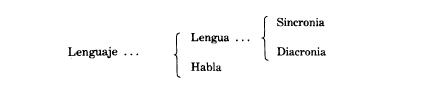
\includegraphics[width=.9\linewidth]{./assets/clasificacion_saussure.png}
\caption{Distinción entre sincronía y diacronía}
\end{figure}

¿Es posible  modelar algorítmicamente  tales conceptos? Según
Jakobson, en el estudio de la \emph{literariedad} se omite el factor emisor
y factor receptor. Tan solo se centra en el mensaje. Representado
 únicamente a través de un \emph{medio} particular: en este caso, la palabra escrita.
Es, por lo tanto,  \emph{factible} que un autómata pueda medir y presentar tales
características. 

\begin{figure}[htbp]
\centering
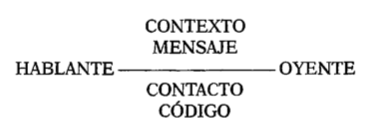
\includegraphics[width=.9\linewidth]{./assets/factores_comunicacion.png}
\caption{Factores de comunicación de Roman Jakobson}
\end{figure}

Saussure ofrece ya un modelo cualitativo muy bien esbozado en teoría,
que es el que luego Jakobson utilizará para definir la literariaded.
Sin embargo, aunque existe un planteamiento cualitativo del problema,
no se halló en la bibliografía consultada un modelo computacional que
modelara el concepto y lo implementara. 

\begin{figure}[htbp]
\centering
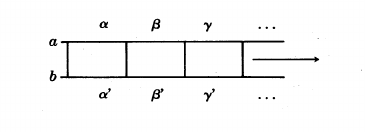
\includegraphics[width=.9\linewidth]{./assets/delimitacion_saussure.png}
\caption{Modelo cualitativo inicial expuesto por Ferdinand De Saussure}
\end{figure}
Preliminarmente, se puede observar que el modelo de Saussure se
fundamenta en una estructura bastante familiar en la computación: la
secuencia. Así, el objetivo de este trabajo es modelar e implementar el
modelo de \emph{literariedad} de Roman Jakobson utilizando redes semánticas
y n-gramas.


\subsection{Justificacón}
\label{sec:orgabc53da}

Si bien existen infinitas operaciones realizables sobre un texto
computarizado, hay pocas que tengan un enfoque de artes liberales u
humanístico. En este enfoque se busca someter a escrutinio los
conceptos del marco teórico, en contraposición a los enfoques
'típicos' --y hoy en día indispensables-- de procesamiento de
lenguaje: extracción de información, clasificación con base a un
modelo predictivo, entre muchos otros.

Más aún, dentro de este subcunjunto reducido, pocos están guiados por
aquello que Gelbuhk llama 'la ciencia fundamental'. A saber, la
linguística. En otras palabras, hay un vacío en el campo de la
linguística computacional en lo que se refiere a modelos que procuran
cuantificar esta perspectiva.

Tal vacío genera que el estudio académico de la literatura no pueda
sustentarse en datos 'duros' o ,por lo menos, cuantitativos propias
del método científico. Por otro lado, los diversas y posibles formas
de calcular la 'creatividad', la 'rima' o la 'belleza' de un texto,
propuesto por otros investigadores, pueden considerarse casuísticos,
acoplados a las objetivos y circunstancias de cada investigación en
particular, desde la perspectiva de la linguística general.

Así, se necesita un modelo de la \emph{literariedad} que exprese
concretamente la metáfora y la metonimia. Bien sea para ampliar las
aplicaciones de la linguistica computacional o para someter a
escrutinio los planteamientos de la teoría.

En esta investigación se formulará y evaluará un modelo para obtener
una medida cuantitativa para el concepto de \emph{literariedad} de Roman
Jakobson utilizando redes semánticas y n-gramas. De este modo, la
presente investigación respondería a la pregunta ¿Cómo medir
computarizadamente la \emph{literariedad} de un texto según el marco de la
lingüística de Jakobson?

\subsubsection{\textbf{Palabras clave:}}
\label{sec:orgd34e673}
NLP, computational linguistics, literariness,literary theory, poetics, theory of formal method

Área de conocimiento:

Lingüística computacional

\subsection{Alcances y delimitaciones:}
\label{sec:orgd0eb2a7}

Para computar una métrica de \emph{literariedad} será necesario comparar
un \emph{corpus objetivo} con respecto a un \emph{corpus de referencia,} este
último representará el ‘uso corriente de la lengua'. La primera
limitación de este trabajo es que no se compilará un corpus propio, sino
que partirá de los de acceso libre. La mayoría de estos se encuentran en
inglés. Por este motivo, el corpus de referencia más a la mano es
WordNet, que al ser una ontología ya contiene las anotaciones necesarias
para mi objetivo. A saber, una lista de sinónimos por palabras. Por otro
lado, el corpus objetivo no tiene que estar anotado (utilizaré un
PlainTextCorpus), pero de algún modo tiene que ser razonable su
comparación con el corpus objetivo. Por ejemplo, los resultados del
modelo serían muy difíciles de evaluar si la relación entre corpus
objetivo y de referencia sobrepasa los 2 siglos, dada la naturaleza
fluida de la lengua.

La segunda limitación concierne a la formulación de los algoritmos en sí
mismos. Me limitaré a formular los modelos más naive posibles. Por
ejemplo, (retomando el ejemplo previo) dada una palabra se considerará
un sinónimo todas las palabras listadas como tal en el corpus de
referencia, sin considerar los sub-problemas que esto podría conllevar.

En general, el alcance de este proyecto es formular e implementar un
modelo general que muestre cómo sería viable implementar el concepto de
\emph{literariedad}, sin ahondar en los detalles que se desprenden de cada
fase del flujo de NLP (por ejemplo, ¿cómo tokenizar?, ¿Qué peso tendrían
las diferentes partes de una oración en el computo final, etc).

\section{OBJETIVO GENERAL}
\label{sec:org51ee356}
Diseñar e implementar un modelo que, dado un corpus de texto, produzca
indicadores para el concepto de \emph{literariedad} que plantea Roman Jakobson.

\section{OBJETIVOS ESPECÍFICOS}
\label{sec:orgb45bbf7}

\begin{enumerate}
\item Construir el corpus necesario para representar el \emph{eje sincrónico}
\item Diseñar e implementar el algoritmo para calcular la \emph{metáfora} sobre un corpus
\item Diseñar e implementar algoritmo para calcular la \emph{metonimia} sobre un corpus
\item Seleccionar y unir los textos que serán procesados (corpus objetivo) por el algoritmo
\item Correr el algoritmo sobre los corpus objetivo
\item Evaluar el algoritmo de manera cuantitativa y cualitativa
\end{enumerate}

\section{MARCO TEÓRICO}
\label{sec:orge6a0cd1}

\subsection{Literariedad}
\label{sec:org5ae25ef}


La \emph{literariedad} es, según Jakobson, la cualidad de un objeto
literario en cuanto tal. Por lo tanto, la \emph{literariedad} no depende de
ningún factor extrínseco, como su emisor, su valor histórico, las
ventas de tal o cual libro, las citaciones, etc. La \emph{literariedad} se
da exclusivamente por atributos propios del fenómeno del lenguaje.

Para analizar la \emph{literariedad}, se deben analizar las dos operaciones
más básicas de la conducta verbal: \emph{la selección} y \emph{la combinación.}


\begin{enumerate}
\item Selección (ver linguística sincrónica):

La selección estudia qué palabra selecciona un hablante entre las
palabras existentes de la lengua, más o menos similares y hasta
cierto punto equivalentes. La selección se basa en la sinonimia o
antonimia de una palabra. En otros términos, en su semántica.
\end{enumerate}



\begin{enumerate}
\item Combinación (ver linguística diacrónica):

La combinación estudia el "entramado de la secuencia" de un
mensaje. Es decir, el mensaje considerado como una secuencia
temporal y/o ordenada de palabras. La combinación se basa en la
proximidad o, en otras palabras, en la relación de una palabra con
la que la sucede o antecede en un mensaje.
\end{enumerate}




\subsection{Poética}
\label{sec:org3034131}
La poética procura responder a la pregunta de ¿qué hace que un
mensaje (verbal o de otra naturaleza) sea una obra de arte? Lidia
principalmente con cuestiones estéticas del lenguaje. Sin embargo,
para hacer un analisis exhaustivo, la poética debe hacer uso de la
linguística, puesto que esta última estudia el lenguaje en todo su
conjunto. La \emph{literariedad} podría, entonces, considerarse un
concepto enmarcado en la poética, porque se preguntá qué hace que
un texto sea literario y por qué es distinto de otro que no lo es.

\subsection{Linguística}
\label{sec:org7c85a53}



La lingüística es la ciencia que estudia el lenguaje.
Tradicionalmente, esta ciencia se subdivide en las ramas de fonética,
fonología, morfología, sintaxis, semántica y pragmática.

La lingüística es un campo de estudio interdisciplinar e involucra
disciplinas heterogéneas como la lógica y la neurolingüistica. Sin
embargo, se considera que hay un núcleo común llamado \emph{linguística
general}.

\begin{enumerate}
\item Lingüística General:

Se conoce como lingüística general al paradigma lingüístico
establecido por Ferdinand De Saussure, también llamado \emph{modelo
diferencial del lenguaje}.

El modelo diferencial se caracteriza porque propone dos ejes
principales existentes en todo fenómeno lingüístico: el \emph{eje de
sincronía} y el \emph{eje de diacronía}.

Estos dos ejes son la base de lo que Jakobson considera \emph{selección} y
\emph{combinación}.
\end{enumerate}


\begin{enumerate}
\item Linguística sincrónica

La linguística sincrónica se ocupa de las
operaciones que realiza un hablante, sean lógicas o psicológicas,
para formar un sistema linguístico (\citeprocitem{1}{De Saussure 1945}). En el
marco de esta investigación el \emph{eje sincrónico} se referirá a las
posibles palabras que un hablante pudo haber seleccionado para
expresar una misma idea.
\end{enumerate}


\begin{enumerate}
\item Linguística diacrónica 

La linguística diacrónica estudia los campos sucesivos en el 
lenguaje, producidos por la actividad constante del \emph{eje 
sincrónico} (\citeprocitem{1}{De Saussure 1945}). En la perspectiva 
 de Jakobson, un \emph{mensaje} tiene en sí mismo un eje 
 diacrónico. Tal eje mide la similaridad entre cada
 término del mensaje entindido como secuencia:"
 \ldots{} para decirlo de un modo más técnico: todo
 secuencia es un símil." (\citeprocitem{2}{Jakobson and Cabello 1981})
\end{enumerate}

\subsection{Lingüística Computacional}
\label{sec:org15d7310}


Es la intersección entre la computación y la lingüística. Por lo
general, se preocupa acerca de cómo procesar automáticamente el
lenguaje material, para lo cual genera modelos lingüísticos sobre los
que luego se pueden definir operaciones comunes [6].


La lingüística computacional es en sí misma un campo amplio y
heterogéneo, pero en términos de este trabajo, me limitaré a señalar
una herramienta:

\begin{enumerate}
\item NLTK
\end{enumerate}

El Natural Language Toolkit (NLTK) es un módulo de Python que ofrece
una interfaz para tareas comunes en la lingüística computacional. La
ventaja principal de NLTK es que se considera a sí mismo un
\emph{toolkit}. Esto significa que no impone una estructura de
procesamiento definida a la vez que ofrece un extenso abanico de
herramientas, tales como: tokenizacion, filtros, generación de
n-gramas, análisis sintáctico de oraciones, entre otras.

\begin{enumerate}
\item Corpus
\end{enumerate}


Un corpus es una colección de textos auténticos que pueden ser leídos
por una máquina. Estos pueden estructurarse de muchas formas,
dependiendo de los objetivos de la investigación [9]. Por ejemplo,
pueden ser aislados (una colección arbitraria), categorizados (una
colección escogida según algún criterio), temporales (una colección
organizada cronológicamente) o solapados (un documento puede
pertenecer a varias colecciones) [10]. Además, el formato del corpus
varía significativamente de acuerdo al objeto de la investigación. Por
ejemplo, si se desea hacer un análisis sintáctico (de la estructura de
una oración), se debe hacer un corpus anotado con POS (Part Of Speech
tag); para hacer un análisis pragmático se utiliza una anotación
pragmática, etc.

\section{MARCO REFERENCIAL}
\label{sec:org9869c3c}

El trabajo de Delmonte [2] presenta a SPARSAR, un sistema para calcular
automáticamente el estilo de la poesía. SPARSAR funciona sobre sistemas
previos del mismo autor, como, por ejemplo, un analizador semántico [7].
Delmonte tiene una larga trayectoria en el modelamiento de conceptos
lingüísticos "difíciles", como la prosodia y la rima en términos
cuantitativos.

El aporte principal de Delmonte fue su innovación al momento de aplicar
herramientas comunes de NLP (tokenizadores, splitters y NER) con el fin
de analizar aspectos estilísticos de un texto. Los modelos de Delmonte
son muy cercanos a la teoría lingüística y propone soluciones a aspectos
complejos del análisis lingüístico. Esta proximidad me llevo a
plantearme la pregunta ¿qué otros aspectos del lenguaje valdría la pena
modelar que aún no hayan sido abordados desde una perspectiva
computacional? Así mismo, Delmonte reporta que hay pocos trabajos en el
área con este mismo enfoque. Esta fue una inspiración para explorar más
en el tema y ofrecer un enfoque distinto, tal como él lo hizo.

Sin embargo, Delmonte no revela detalles de implementación de sus sis-
temas en los artículos revisados. Además, sus sistemas tienen una
alcance mucho mayor que el dispuesto para este trabajo, por lo que para
mayores detalles tuve que referirme a otros trabajos.

El trabajo de [5] establece una métrica para medir el grado de
creatividad en la poesía, basándose en qué tanto de la rima se conserva
en la traducción de un poema con respecto al original. Tomé de Zuñiga la
idea de establecer una métrica para un aspecto tradicionalmente
cualitativo (la creatividad). Lo que diferencia este trabajo del de
Delmonte, es su aproximación matemática. Particularmente, Zuñiga ofreció
una forma naive de calcular similitud en rima, sin necesidad de recurrir
a construcciones que requieren de recursos léxicos complejos como una
ontología para fonemas, etc.

Por último, el trabajo de [8] es una tesis de pregrado sobre el cálculo
del estilo de la poesía desde una perspectiva estadística. Kaplan fue
una inspiración para Delmonte, por lo tanto debía formar parte de mi
revisión bibliográfica. El aporte principal a mi trabajo ha sido tener
una serie de ope- raciones como referencia. Por ejemplo, para modelar
aspectos ortográficos, sintácticos y fonémicos, entre otros.

\section{DISEÑO METODOLÓGICO}
\label{sec:org243191d}
\subsection{Entendimiento del negocio}
\label{sec:orgec2bbae}
(Me pareció que esto no aplica. Discutir con profesor. Propongo esto otro)

Lo otro sería explicar los posibles usos (posibles clientes) de mi modelo
\begin{figure}[htbp]
\centering
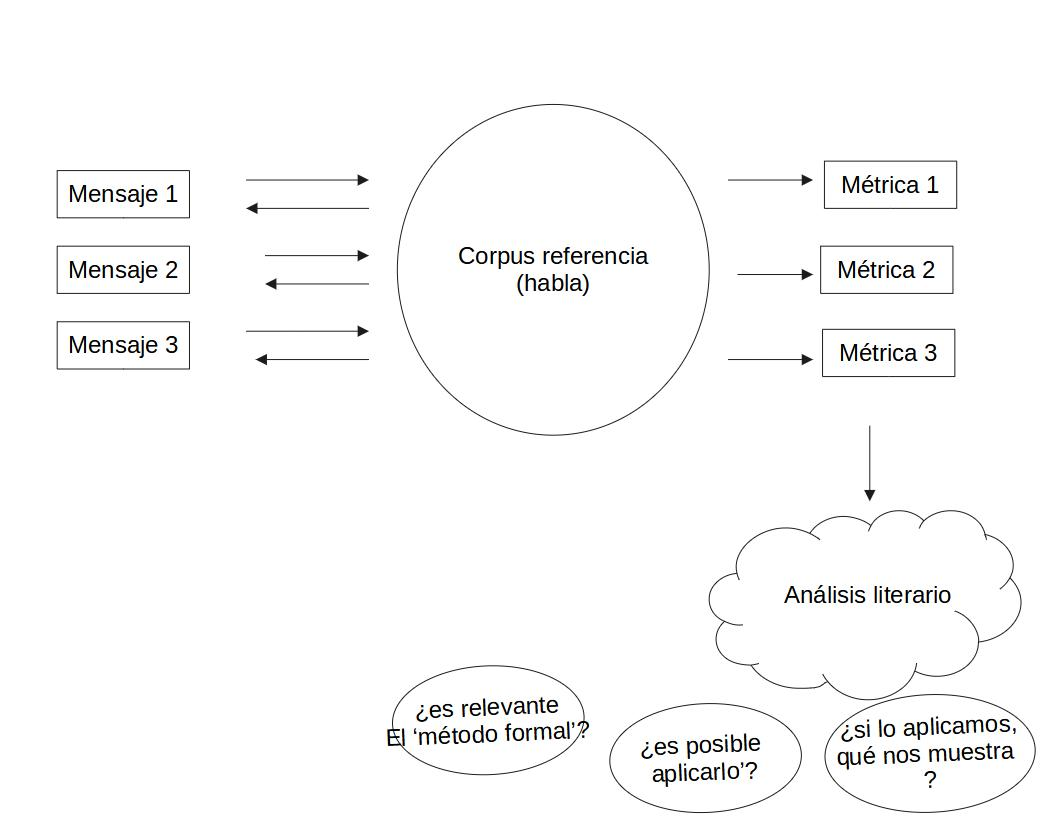
\includegraphics[width=.9\linewidth]{./assets/posibles_usos.jpg}
\caption{Entradas y salidas del algoritmo}
\end{figure}

\subsection{Entendimiento de los datos}
\label{sec:orge6df6e3}

\begin{quote}
The data understanding phase of CRISP-DM involves taking a closer
look at the data available for mining. This step is critical in
avoiding unexpected problems during the next phase--data
preparation--which is typically the longest part of a project.
\end{quote}

\subsubsection{Los recursos lexicos}
\label{sec:org7ff7aea}

\begin{figure}[htbp]
\centering
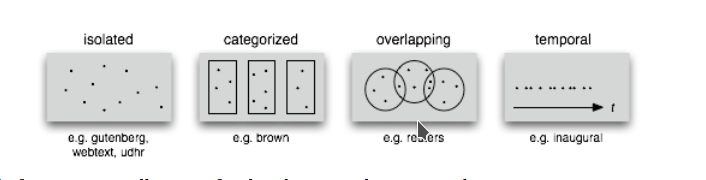
\includegraphics[width=.9\linewidth]{./assets/estructuras_de_corpus.png}
\caption{Diferentes estructuras de corpus}
\end{figure}

\begin{enumerate}
\item Corpus de referencia
\label{sec:org58d1960}
El corpus de referencia es Wordnet. 
\item Corpus objetivo
\label{sec:org885a2ca}
El corpus escogido fue el corpus de Brown porque cumplía con las siguientes criterios:
\begin{enumerate}
\item La lengua inglesa tiene una correspondiente red semántica
\item Esta categorizado, por lo que se espera observar diferencias significativas en el resultado de su procesamiento
\item Es fácilmente accesible a través de Python
\end{enumerate}
\end{enumerate}

\subsubsection{La red semántica y similaridad con Saussure}
\label{sec:org290b068}
\subsubsection{Por qué utilizo el Brown Corpus}
\label{sec:orgd320abc}
\subsection{Preparación de los datos}
\label{sec:org3fe2700}

\begin{verbatim}
Depending on your organization and its goals, data preparation typically involves the following tasks:

Merging data sets and/or records
Selecting a sample subset of data
Aggregating records
Deriving new attributes
Sorting the data for modeling
Removing or replacing blank or missing values
Splitting into training and test data sets

\end{verbatim}
\subsection{Modelamiento}
\label{sec:orge203b5c}
\subsubsection{Selecting a modeling technique (no tengo, estoy traduciendo un modelo cualitativo --investigacion mixta--)}
\label{sec:org33cba80}
\subsubsection{Generating a test desing}
\label{sec:org4e4267f}


\begin{itemize}
\item Describing the criteria for "goodness" of a model
\item Defining the data on which these criteria will be tested
\end{itemize}
\begin{enumerate}
\item Sampleo de la muestra
\label{sec:org4dd3208}
\begin{itemize}
\item qué textos voy a someter a procesamiento
\item por qué escogí estos textos en particular
\end{itemize}
\end{enumerate}
\subsubsection{Building the models}
\label{sec:org281aacf}
\begin{enumerate}
\item Presentacion de las ecuaciones
\label{sec:org0ead8e8}

      \begin{equation}
mensaje = \{ w_1, w_2, w_3, \dots , w_j \} \\
\end{equation}

\begin{equation}
vector\ semantico(w) = \{s_1, s_2, s_3, \dots, s_j \} \\
\end{equation}

\begin{equation}
uso(w) = \frac{freq(w)}{freqMedia}
\end{equation}

\begin{equation}
freqMedia = \mu(freq(corpora\ ref)
\end{equation}

\begin{equation}
indice\ metaforico(mensaje) =  \Sigma_i^j \frac{uso(w_i)}{\mu( vector\ semantico(w_i))}
\end{equation}


\begin{equation}
N = \{n_1, n_2, n_3, \dots , n_j\}
\end{equation}

\begin{equation}
met(n) = \frac{letras\ iguales}{ set(letras(n_i1) + letras(n_i2)}
\end{equation}

\begin{equation}
indice\ metonimia = \Sigma_i^j met(n_i)
\end{equation}

\item Procedimientos para indicadores
\label{sec:orgf5e9d0a}
\begin{figure}[htbp]
\centering
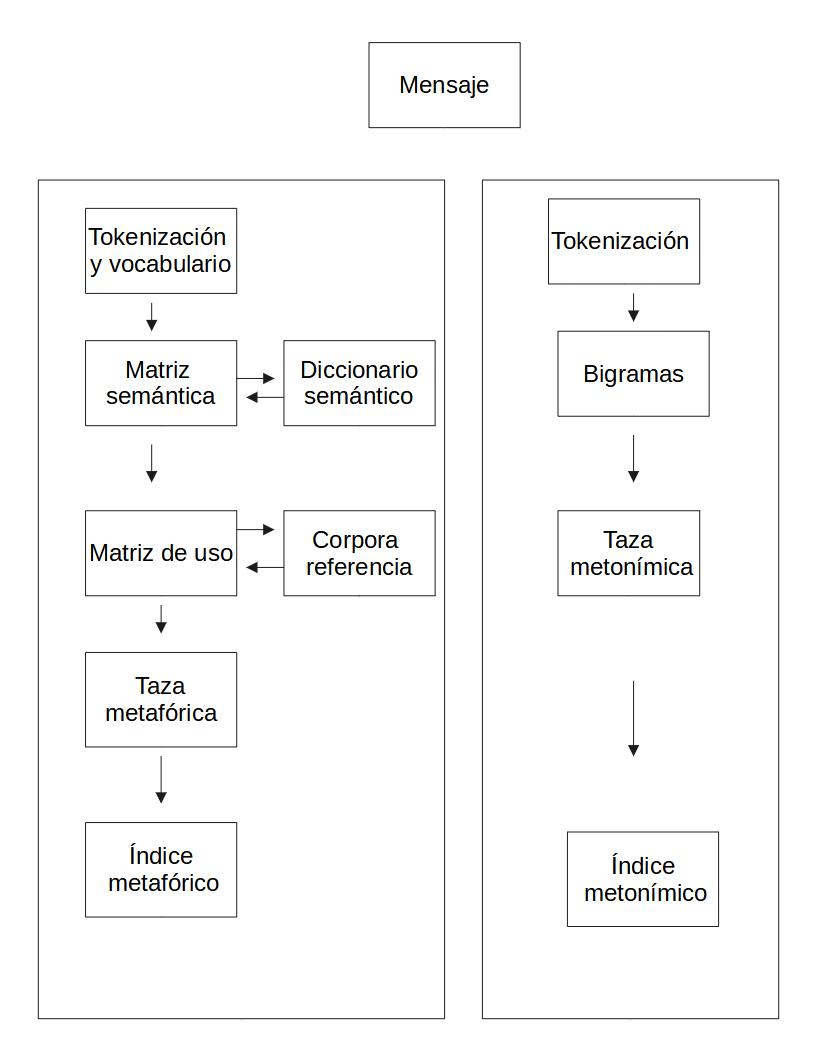
\includegraphics[width=.9\linewidth]{./assets/metodologia.jpg}
\caption{Procesamiento de corpus objetivo}
\end{figure}   
\item Índice Metafórico
\label{sec:orga5dfd76}
\item Matriz semántica
\label{sec:org9f0941a}


\item Matriz de uso
\label{sec:org954421d}

\begin{figure}[htbp]
\centering
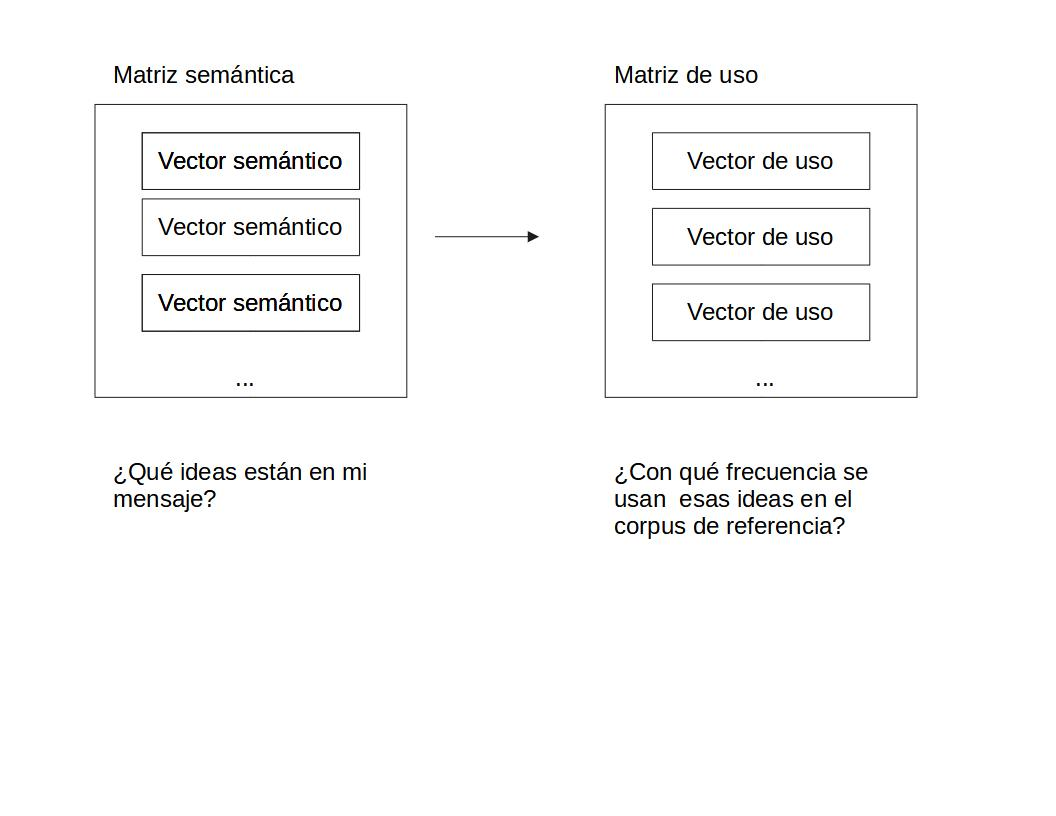
\includegraphics[width=.9\linewidth]{./assets/matrices.jpg}
\caption{Abstracciones necesarias para el índice metafórico}
\end{figure}

\item Índice Metonímico
\label{sec:orgb97d446}
\begin{figure}[htbp]
\centering
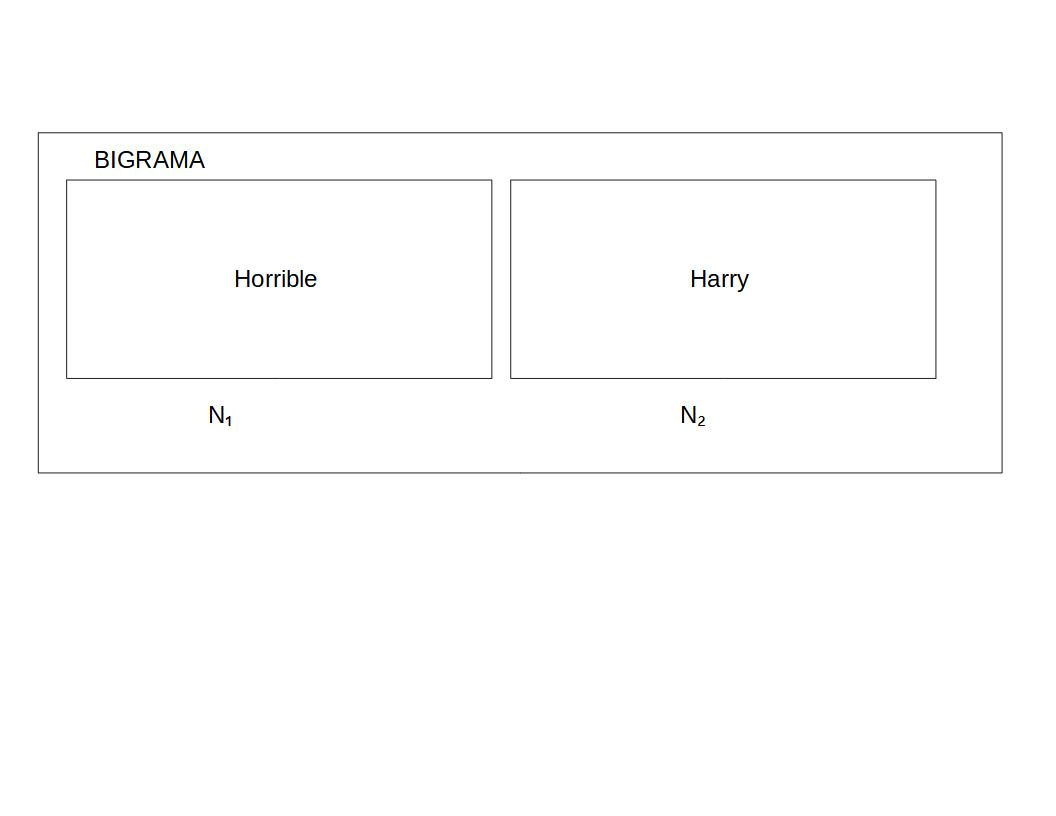
\includegraphics[width=.9\linewidth]{./assets/metonimia.jpg}
\caption{Abstraccciones necesarias para el indice metonímico}
\end{figure}
\end{enumerate}

\subsection{Despliegue (los notebooks?? creo que no hay despliege)}
\label{sec:org7f9d3ae}

\begin{quote}
Deployment is the process of using your new insights to make
improvements within your organization. This can mean a formal
integration such as the implementation of a IBM® SPSS® Modeler model
producing churn scores that are then read into a data
warehouse. Alternatively, deployment can mean that you use the
insights gained from data mining to elicit change in your
organization. For example, perhaps you discovered alarming patterns in
your data indicating a shift in behavior for customers over the age
of 30. These results may not be formally integrated into your
information systems, but they will undoubtedly be useful for planning
and making marketing decisions.
\end{quote}
\section{CONCLUSIONES (Creo que esto se solapa con lo que crisp-dm llama despliege)}
\label{sec:org63a88cd}

\section{BIBLIOGRAFÍA}
\label{sec:org926dff5}

[1]  L. Danlos, “The linguistic basis of text generation,” in
Proceedings of the third conference on European chapter of the
Association for Computatio- nal Linguistics, pp. 1--1, 1987.

[2]  R. Delmonte, “Computing poetry style.,” in ESSEM@ AI* IA, pp. 148--
155, 2013.

[3]  B. Eijembaum, “La teoría del"método formal",” in Textos de teorías
y crítica literarias:(del formalismo a los estudios postcoloniales), pp.
33-- 62, Anthropos, 2010.

[4]  R. Jakobson and A. M. G. Cabello, Lingüística y poética. Cátedra
España, 1981.

[5]  D. F. Zuñiga, T. Amido, and J. E. Camargo, “Automatic computation
of poetic creativity in parallel corpora,” in Colombian Conference on
Computing, pp. 710--720, Springer, 2017.

[6]  I. A. Bolshakov and A. Gelbukh, Computational Linguistics: Models,
Re- sources, Applications. Mexico City: Centro de Investigacio ́øn en
Compu- taci ́øn, Instituto Polit ́cnico Nacional, 1981.

[7]  R. Delmonte, S. Tonelli, M. A. P. Boniforti, and A. Bristot,
“Venses--a linguistically-based system for semantic evaluation,” in
Machine Learning Challenges Workshop, pp. 344--371, Springer, 2005.

[8]  D. Kaplan, “Computational analysis and visualized comparison of
style in american poetry,” Unpublished undergraduate thesis, 2006.

[9] Indurkhya, N., \& Damerau, F. J. “/Handbook of natural language
processing/ (Vol. 2)”. CRC Press, 2010


[10] Bird, Steven, et al. Natural Language Processing with Python.
O'Reilly Media, 2009.




\hypertarget{citeproc_bib_item_1}{De Saussure, Ferdinand. 1945. “Curso de Lingü\’ıstica General.” \textit{Buenos Aires: Losada. Original de Ferdinand de}.}

\hypertarget{citeproc_bib_item_2}{Jakobson, Roman, and Ana Mar\’ıa Gutiérrez Cabello. 1981. \textit{Lingü\’ıstica Y Poética}. Cátedra España.}
\end{document}